\documentclass[11pt,a4paper]{article}

% ---------------------------------------------------------------
% Packages
% ---------------------------------------------------------------
\usepackage[utf8]{inputenc}
\usepackage[T1]{fontenc}
\usepackage{lmodern}
\usepackage[margin=1in]{geometry}
\usepackage{amsmath, amssymb, amsthm, mathtools}
\usepackage{graphicx}
\usepackage{booktabs}
\usepackage{multirow}
\usepackage{array}
\usepackage[expansion=false]{microtype}
\usepackage{listings}
\usepackage{xcolor}
\usepackage{textcomp}
\usepackage{enumitem}
\usepackage{tabularx}
\usepackage{hyperref}
\hypersetup{colorlinks=true, linkcolor=blue!50!black, citecolor=blue!50!black, urlcolor=blue!50!black}

\graphicspath{{figures/}}
\setlength{\emergencystretch}{2em}

\lstdefinestyle{pystyle}{
    language=Python,
    basicstyle=\ttfamily\footnotesize,
    keywordstyle=\color{blue},
    commentstyle=\color{gray},
    stringstyle=\color{teal},
    showstringspaces=false,
    breaklines=true,
    frame=single,
    tabsize=4
}

% ---------------------------------------------------------------
% Theorem environments and macros
% ---------------------------------------------------------------
\theoremstyle{plain}
\newtheorem{theorem}{Theorem}[section]
\newtheorem{proposition}[theorem]{Proposition}
\newtheorem{lemma}[theorem]{Lemma}
\theoremstyle{definition}
\newtheorem{definition}[theorem]{Definition}
\newtheorem{remark}[theorem]{Remark}

\newcommand{\dd}{\mathrm{d}}
\newcommand{\E}{\mathbb{E}}
\newcommand{\Q}{\mathbb{Q}}
\newcommand{\R}{\mathbb{R}}
\newcommand{\F}{\mathcal{F}}
\newcommand{\N}{\mathcal{N}}
\newcommand{\bp}{\,\mathrm{bp}}
\newcommand{\eur}{\text{\texteuro}}
\DeclareMathOperator{\Var}{Var}
\DeclareMathOperator{\Cov}{Cov}

\title{\textbf{The One-Factor Hull--White Model:\\
Theory, Pricing, Calibration, Strengths and Limitations}}
\author{\textbf{Elias Benguedda}}
\date{October 2026}

\begin{document}

\maketitle

\begin{abstract}
This paper gives a self-contained presentation of the one-factor Hull--White model, the extended Vasicek short-rate model $\dd r(t)=(\theta(t)-a\,r(t))\,\dd t+\sigma\,\dd W(t)$ that remains, more than thirty years after its introduction, the workhorse of interest rate desks for callable and Bermudan products and for the simulation of rates in XVA engines. We derive the fit to the initial term structure, the decomposition $r=x+\alpha$ into a centred Ornstein--Uhlenbeck factor and a deterministic shift, the affine zero-coupon bond formula, the closed forms for zero-coupon bond options, caps, floors and European swaptions (Jamshidian's decomposition), and the exact joint simulation of the short rate and its integral.

Every result is illustrated with the Python implementation of this repository on the EURIBOR 6M curve of 12 February 2025 and on illustrative normal volatilities. A Monte Carlo martingale test reproduces the initial discount factors within the statistical error. A global calibration to 25 at-the-money swaptions leaves a root-mean-square error of $2.9\bp$ of normal volatility and cannot reproduce the hump of the volatility surface, while a co-terminal calibration fits 9 swaptions within $1\bp$. On a $2\text{y}\times8\text{y}$ Bermudan swaption, three calibrations with the same quality of fit on the European swaptions give Bermudan prices that differ by $9\%$: the mean reversion, which European prices barely constrain, drives the value of the switch option. We conclude with a structured discussion of the advantages of the model (tractability, exact fit, speed, transparency) and of its drawbacks (one factor, Gaussian rates, no smile, rigid volatility structure), together with the standard extensions. This paper is linked to my GitHub, which can be found on my portfolio\footnote{\url{https://portfolio-eliasbenguedda.fr}}, and all scripts are available in the same repository.
\end{abstract}

\clearpage

\tableofcontents
\newpage

% ===============================================================
\section{Introduction}
\label{sec:intro}
% ===============================================================

\subsection{Motivation}
Interest rate derivatives are written on the whole term structure, not on a single asset. A model must therefore describe the joint random evolution of all the discount factors $P(t,T)$, $T\geq t$, in a way that is free of arbitrage, consistent with today's curve, and simple enough to price and hedge thousands of trades every day. Short-rate models achieve this by modelling a single quantity, the instantaneous rate $r(t)$, from which every bond price follows by risk-neutral valuation,
\begin{equation}
    P(t,T)=\E^{\Q}\Bigl[\exp\Bigl(-\int_t^T r(s)\,\dd s\Bigr)\Bigm|\F_t\Bigr].
    \label{eq:bond-def}
\end{equation}

The first such models, Vasicek~\cite{vasicek} (Gaussian, mean reverting) and Cox--Ingersoll--Ross~\cite{cir} (square root), are \emph{equilibrium} models: with constant parameters they produce their own yield curve, which never matches the market curve exactly. For pricing, this is unacceptable, since a model that misprices a zero-coupon bond misprices every swap. Ho and Lee~\cite{holee} introduced the first \emph{no-arbitrage} model, which takes the initial curve as an input, but without mean reversion. Hull and White~\cite{hullwhite} combined the two ideas in 1990: they made the drift of the Vasicek model time dependent and chose it so that the model reprices the initial curve exactly. The result, the one-factor Hull--White model (HW1F), keeps all the analytical tractability of Vasicek and adds exact consistency with the market.

\subsection{Why the model still matters}
Despite the development of the LIBOR Market Model, SABR and multi-factor models, HW1F remains ubiquitous:
\begin{itemize}
    \item it is the reference model for Bermudan swaptions and callable bonds, where an exercise decision on a low-dimensional state is needed;
    \item it is the standard rate model of XVA and counterparty risk engines, where millions of paths of the whole curve must be generated quickly;
    \item it is used as a control variate, a benchmark, and the building block of hybrid models (rates--equity, rates--FX, rates--credit);
    \item its linear Gaussian structure makes the role of each parameter transparent, which is valuable for risk management and model validation.
\end{itemize}

\subsection{Organization of the paper}
Section~\ref{sec:prelim} fixes notation. Section~\ref{sec:model} defines the model and derives the fit to the initial curve. Section~\ref{sec:bonds} derives bond prices and the induced dynamics of forward rates. Section~\ref{sec:pricing} gives the pricing formulas for options and the numerical methods for early exercise. Section~\ref{sec:calibration} discusses calibration. Section~\ref{sec:numerics} illustrates the model with the implementation of this repository. Sections~\ref{sec:advantages} and~\ref{sec:drawbacks} discuss the advantages and the drawbacks of the model, and Section~\ref{sec:extensions} reviews its extensions. Section~\ref{sec:conclusion} concludes. The appendices contain proofs, code excerpts and the notation.

\clearpage
% ===============================================================
\section{Preliminaries and Notation}
\label{sec:prelim}
% ===============================================================

We work on a filtered probability space $(\Omega,\F,(\F_t)_{t\geq0},\Q)$, where $\Q$ is the risk-neutral measure associated with the bank account
\begin{equation}
    \beta(t)=\exp\Bigl(\int_0^t r(s)\,\dd s\Bigr),
    \qquad
    D(t,T)=\frac{\beta(t)}{\beta(T)}=\exp\Bigl(-\int_t^T r(s)\,\dd s\Bigr).
\end{equation}
The price at $t$ of an attainable claim paying $H$ at $T$ is $\E^\Q[D(t,T)H\mid\F_t]$; in particular the zero-coupon bond $P(t,T)$ is given by~\eqref{eq:bond-def}, with $P(T,T)=1$.

\paragraph{Forward rates.} The instantaneous forward rate and the simply compounded forward rate over $[T_1,T_2]$ are
\begin{equation}
    f(t,T)=-\frac{\partial\ln P(t,T)}{\partial T},
    \qquad
    F(t;T_1,T_2)=\frac{1}{T_2-T_1}\Bigl(\frac{P(t,T_1)}{P(t,T_2)}-1\Bigr),
    \label{eq:forwards}
\end{equation}
and $r(t)=f(t,t)$. The market curve today is the function $T\mapsto P^M(0,T)$, with instantaneous forward $f^M(0,T)$. In this paper it is built from the EURIBOR 6M zero-coupon rates of 12 February 2025 with the monotone convex interpolation of Hagan and West~\cite{haganwest2006}, as in the yield curve paper of this portfolio. To lighten notation, we write $P(0,T)$ and $f(0,T)$ for the market quantities.

\paragraph{Forward measure.} For a maturity $T$, the $T$-forward measure $\Q^T$ is the measure associated with the numéraire $P(t,T)$:
\begin{equation}
    \frac{\dd\Q^T}{\dd\Q}\Big|_{\F_t}=\frac{P(t,T)}{P(0,T)\,\beta(t)}.
\end{equation}
Under $\Q^T$, the price of any asset divided by $P(t,T)$ is a martingale, so that the price of a claim $H$ paid at $T$ is $P(0,T)\,\E^{T}[H]$. This change of numéraire~\cite{geman} is the key tool of Section~\ref{sec:pricing}.

\paragraph{Swaps.} A payer swap starting at $T_0$ with fixed payment dates $T_1<\dots<T_N$, accruals $\delta_i=T_i-T_{i-1}$ and fixed rate $K$ is worth, in a single-curve framework,
\begin{equation}
    V^{\text{swap}}(t)=P(t,T_0)-P(t,T_N)-K\sum_{i=1}^N\delta_iP(t,T_i)
    =A(t)\bigl(S(t)-K\bigr),
    \label{eq:swap}
\end{equation}
where $A(t)=\sum_i\delta_iP(t,T_i)$ is the annuity and $S(t)=(P(t,T_0)-P(t,T_N))/A(t)$ the forward swap rate.

\clearpage
% ===============================================================
\section{The Model}
\label{sec:model}
% ===============================================================

\subsection{Definition}
\begin{definition}[One-factor Hull--White model]
Under the risk-neutral measure $\Q$, the short rate follows
\begin{equation}
    \dd r(t)=\bigl(\theta(t)-a\,r(t)\bigr)\,\dd t+\sigma\,\dd W(t),
    \qquad r(0)=f(0,0),
    \label{eq:hw}
\end{equation}
where $W$ is a standard Brownian motion, $a>0$ is the speed of mean reversion, $\sigma>0$ the (absolute, or normal) volatility of the short rate, and $\theta$ a deterministic function of time chosen so that the model reproduces the initial curve $T\mapsto P(0,T)$.
\end{definition}

Rewriting the drift as $a\,(\theta(t)/a-r(t))$ shows the interpretation: the short rate is pulled towards a time-dependent level $\theta(t)/a$ at speed $a$. The characteristic time of the mean reversion is $1/a$, and its half-life $\ln 2/a$: with $a=3\%$, a deviation of the short rate from its mean is halved in about 23 years; with $a=10\%$, in about 7 years. The parameter $\sigma$ is expressed in rate units per square root of year: $\sigma=0.0085$ means $85\bp$ per year, the order of magnitude of EUR normal volatilities.

With $\theta$ constant, \eqref{eq:hw} is the Vasicek model; with $a=0$, it is the Ho--Lee model. The original paper of Hull and White~\cite{hullwhite} also allows $a$ and $\sigma$ to depend on time; we return to this extension in Section~\ref{sec:extensions}.

\subsection{Explicit solution}
Equation~\eqref{eq:hw} is linear. Applying Itô's formula to $e^{at}r(t)$ gives, for $s\leq t$,
\begin{equation}
    r(t)=r(s)\,e^{-a(t-s)}+\int_s^t e^{-a(t-u)}\theta(u)\,\dd u+\sigma\int_s^te^{-a(t-u)}\,\dd W(u).
    \label{eq:solution}
\end{equation}
The stochastic integral has a deterministic integrand, hence is Gaussian. Conditionally on $\F_s$, $r(t)$ is therefore normally distributed, with
\begin{equation}
    \E[r(t)\mid\F_s]=r(s)\,e^{-a(t-s)}+\int_s^te^{-a(t-u)}\theta(u)\,\dd u,
    \qquad
    \Var[r(t)\mid\F_s]=\frac{\sigma^2}{2a}\bigl(1-e^{-2a(t-s)}\bigr).
    \label{eq:moments}
\end{equation}
The variance grows like $\sigma^2(t-s)$ for short horizons, as in a Brownian motion, and converges to the stationary level $\sigma^2/(2a)$ for long horizons: mean reversion bounds the dispersion of the short rate. With $a=3\%$ and $\sigma=85\bp$, the stationary standard deviation is $\sigma/\sqrt{2a}\approx3.5\%$.

\subsection{Fitting the initial term structure}
\begin{proposition}[Choice of $\theta$]\label{prop:theta}
The model~\eqref{eq:hw} reproduces the initial discount curve, $P^{HW}(0,T)=P(0,T)$ for all $T$, if and only if
\begin{equation}
    \theta(t)=\frac{\partial f(0,t)}{\partial T}+a\,f(0,t)+\frac{\sigma^2}{2a}\bigl(1-e^{-2at}\bigr).
    \label{eq:theta}
\end{equation}
\end{proposition}
The proof is given in Appendix~\ref{app:proofs}. The three terms of~\eqref{eq:theta} have a clear meaning: the first follows the slope of the forward curve, the second compensates the mean reversion, and the third is a convexity correction. Because $\exp(-\int r)$ is a convex function of the rates, the volatility increases bond prices (Jensen's inequality); the drift must be raised to compensate, more so for large $\sigma$ and long maturities.

\begin{remark}[Smoothness of the curve]\label{rem:smooth}
Formula~\eqref{eq:theta} involves the \emph{derivative} of the instantaneous forward curve, which is itself the derivative of $\ln P(0,T)$. Any irregularity of the curve construction (a kink of the zero curve, a jump of the forward curve) is amplified twice in $\theta$. This is a strong argument for a smooth interpolation with a continuous forward curve, such as monotone convex, and for never using $\theta$ directly in a numerical scheme: the shift formulation below avoids the derivative altogether.
\end{remark}

\subsection{Decomposition into a centred factor and a deterministic shift}
The most convenient way to implement the model, used in the code of this repository and recommended by Brigo and Mercurio~\cite{brigomercurio}, is to separate the randomness from the fit to the curve.

\begin{proposition}[Shift decomposition]\label{prop:shift}
Let $x$ be the centred Ornstein--Uhlenbeck process
\begin{equation}
    \dd x(t)=-a\,x(t)\,\dd t+\sigma\,\dd W(t),\qquad x(0)=0,
    \label{eq:ou}
\end{equation}
and define
\begin{equation}
    \alpha(t)=f(0,t)+\frac{\sigma^2}{2a^2}\bigl(1-e^{-at}\bigr)^2.
    \label{eq:alpha}
\end{equation}
Then $r(t)=x(t)+\alpha(t)$ solves~\eqref{eq:hw} with $\theta$ given by~\eqref{eq:theta}.
\end{proposition}
\begin{proof}
$\dd r=\dd x+\alpha'(t)\,\dd t=\bigl(\alpha'(t)+a\alpha(t)-a\,r(t)\bigr)\dd t+\sigma\,\dd W$, so $r$ follows~\eqref{eq:hw} with $\theta=\alpha'+a\alpha$. Differentiating~\eqref{eq:alpha},
$\alpha'+a\alpha=\partial_Tf(0,t)+af(0,t)+\frac{\sigma^2}{a}(1-e^{-at})e^{-at}+\frac{\sigma^2}{2a}(1-e^{-at})^2$, and the last two terms sum to $\frac{\sigma^2}{2a}(1-e^{-at})(1+e^{-at})=\frac{\sigma^2}{2a}(1-e^{-2at})$.
\end{proof}

The state variable $x$ does not depend on the curve; the curve only enters through $\alpha$, which involves $f(0,t)$ but not its derivative. In particular
\begin{equation}
    \E[r(t)]=\alpha(t),\qquad
    x(t)\mid\F_s\sim\N\Bigl(x(s)e^{-a(t-s)},\ \frac{\sigma^2}{2a}\bigl(1-e^{-2a(t-s)}\bigr)\Bigr).
    \label{eq:x-law}
\end{equation}
The expected short rate is the forward rate plus a convexity term that is of order $\sigma^2t^2/2$ for small $at$. With $\sigma=85\bp$, this term is $8.6\bp$ at 5 years and $33\bp$ at 10 years for $a=1\%$, and smaller for stronger mean reversion (Figure~\ref{fig:alpha} in Section~\ref{sec:numerics}). The expected short rate is \emph{not} the forward rate: the forward is the expectation of the future short rate under the forward measure, not under $\Q$.

\clearpage
% ===============================================================
\section{Bond Prices and Term-Structure Dynamics}
\label{sec:bonds}
% ===============================================================

\subsection{The affine bond formula}
\begin{theorem}[Zero-coupon bond]\label{thm:bond}
In the Hull--White model fitted to the curve,
\begin{equation}
    P(t,T)=\frac{P(0,T)}{P(0,t)}\exp\Bigl(-B(t,T)\,x(t)-V(t,T)\Bigr),
    \qquad
    B(t,T)=\frac{1-e^{-a(T-t)}}{a},
    \label{eq:bond}
\end{equation}
with the deterministic convexity term
\begin{equation}
    V(t,T)=\frac{\sigma^2}{2a^2}\bigl(1-e^{-at}\bigr)^2B(t,T)+\frac{\sigma^2}{4a}\bigl(1-e^{-2at}\bigr)B(t,T)^2.
    \label{eq:V}
\end{equation}
Equivalently, in terms of the short rate, $P(t,T)=A(t,T)\,e^{-B(t,T)r(t)}$ with
\begin{equation}
    A(t,T)=\frac{P(0,T)}{P(0,t)}\exp\Bigl(B(t,T)f(0,t)-\frac{\sigma^2}{4a}\bigl(1-e^{-2at}\bigr)B(t,T)^2\Bigr).
    \label{eq:A}
\end{equation}
\end{theorem}
The proof is in Appendix~\ref{app:proofs}. The model is \emph{affine}: the log of every bond price is an affine function of the single state variable. Three consequences follow immediately.
\begin{enumerate}[label=(\roman*)]
    \item The whole curve at a future date $t$ is a deterministic function of one number, $x(t)$. Simulating the curve costs as much as simulating a scalar.
    \item Zero-coupon yields $R(t,T)=-\ln P(t,T)/(T-t)$ are affine in $x(t)$, hence Gaussian, and negative values have positive probability.
    \item At $t=0$, $x(0)=0$ and $V(0,T)=0$, so $P(0,T)$ is recovered exactly, whatever $a$ and $\sigma$.
\end{enumerate}

\subsection{Bond and forward rate dynamics}
Applying Itô's formula to~\eqref{eq:bond}, the bond dynamics under $\Q$ are
\begin{equation}
    \frac{\dd P(t,T)}{P(t,T)}=r(t)\,\dd t-\sigma B(t,T)\,\dd W(t).
    \label{eq:bond-dyn}
\end{equation}
The bond volatility $\sigma B(t,T)$ increases with the time to maturity and saturates at $\sigma/a$: mean reversion limits the price volatility of long bonds. Differentiating $-\ln P(t,T)$ in $T$ gives the dynamics of the instantaneous forward rates,
\begin{equation}
    \dd f(t,T)=\sigma^2e^{-a(T-t)}B(t,T)\,\dd t+\sigma e^{-a(T-t)}\,\dd W(t).
    \label{eq:fwd-dyn}
\end{equation}
In the Heath--Jarrow--Morton framework~\cite{hjm}, HW1F is exactly the model with the separable forward volatility $\sigma_f(t,T)=\sigma e^{-a(T-t)}$, and the drift in~\eqref{eq:fwd-dyn} is the HJM no-arbitrage drift $\sigma_f(t,T)\int_t^T\sigma_f(t,u)\,\dd u$. This separability is what makes the model Markovian in a single state variable.

\subsection{Interpretation of the parameters}
Equation~\eqref{eq:fwd-dyn} gives the clearest reading of the two parameters.
\begin{itemize}
    \item $\sigma$ is the normal volatility of the short end of the curve. It sets the overall level of option prices.
    \item $a$ controls how the volatility decays along the curve: a forward rate of maturity $T-t$ has volatility $\sigma e^{-a(T-t)}$. With $a=0$ (Ho--Lee), all forward rates move by the same amount (parallel shifts); with $a>0$, long rates move less than short rates. The yield of maturity $\tau$ has instantaneous volatility $\sigma B(t,t+\tau)/\tau$.
    \item Since a single Brownian motion drives everything, all rates are \emph{instantaneously perfectly correlated}: $a$ does not change the correlation between rates, it only changes the relative size of their moves. However, $a$ governs the \emph{intertemporal} correlation: the correlation between $x(s)$ and $x(t)$ for $s<t$ is $e^{-a(t-s)}\sqrt{(1-e^{-2as})/(1-e^{-2at})}$, which decreases with $a$. This is the quantity that matters for products with several exercise dates (Section~\ref{sec:bermudan-num}).
\end{itemize}

\clearpage
% ===============================================================
\section{Pricing of Derivatives}
\label{sec:pricing}
% ===============================================================

\subsection{Dynamics under the forward measure}
By Girsanov's theorem and~\eqref{eq:bond-dyn}, $W^T(t)=W(t)+\sigma\int_0^tB(s,T)\,\dd s$ is a Brownian motion under $\Q^T$, and
\begin{equation}
    \dd x(t)=\bigl(-a\,x(t)-\sigma^2B(t,T)\bigr)\,\dd t+\sigma\,\dd W^T(t).
    \label{eq:x-forward}
\end{equation}
The state variable remains Gaussian under every forward measure, with the same variance and a shifted mean. Hence every bond price $P(T,S)$ is lognormal under $\Q^T$, and options on bonds have Black--Scholes-type closed forms.

\subsection{Options on zero-coupon bonds}
\begin{proposition}[Zero-coupon bond option]\label{prop:zbo}
The price at time $0$ of a European call of expiry $T$ and strike $X$ on the zero-coupon bond $P(T,S)$, $S>T$, is
\begin{equation}
    \mathrm{ZBC}(0,T,S,X)=P(0,S)\,\Phi(h)-X\,P(0,T)\,\Phi(h-\sigma_P),
    \label{eq:zbc}
\end{equation}
and the price of the put is $\mathrm{ZBP}(0,T,S,X)=X\,P(0,T)\,\Phi(-h+\sigma_P)-P(0,S)\,\Phi(-h)$, where $\Phi$ is the standard normal distribution function and
\begin{equation}
    \sigma_P=\sigma\sqrt{\frac{1-e^{-2aT}}{2a}}\,B(T,S),
    \qquad
    h=\frac{1}{\sigma_P}\ln\frac{P(0,S)}{X\,P(0,T)}+\frac{\sigma_P}{2}.
    \label{eq:sigmap}
\end{equation}
\end{proposition}
\begin{proof}[Sketch]
Under $\Q^T$, the forward bond price $P(t,S)/P(t,T)$ is a martingale with initial value $P(0,S)/P(0,T)$; by~\eqref{eq:bond} it is lognormal at $t=T$ with log-variance $B(T,S)^2\Var[x(T)]=\sigma_P^2$. The price $P(0,T)\,\E^T[(P(T,S)-X)^+]$ is then given by Black's formula.
\end{proof}

\subsection{Caps and floors}
A caplet on $[T_{i-1},T_i]$ with accrual $\tau_i$ pays $\tau_i(F(T_{i-1};T_{i-1},T_i)-K)^+$ at $T_i$. Its value at $T_{i-1}$ is $(1+K\tau_i)\,(1/(1+K\tau_i)-P(T_{i-1},T_i))^+$, a put on a zero-coupon bond. Hence
\begin{equation}
\begin{aligned}
    \mathrm{Caplet}_i&=(1+K\tau_i)\,\mathrm{ZBP}\Bigl(0,T_{i-1},T_i,\frac{1}{1+K\tau_i}\Bigr),\\
    \mathrm{Floorlet}_i&=(1+K\tau_i)\,\mathrm{ZBC}\Bigl(0,T_{i-1},T_i,\frac{1}{1+K\tau_i}\Bigr),
\end{aligned}
    \label{eq:caplet}
\end{equation}
and a cap is the sum of its caplets. This is the formula implemented in \texttt{HullWhite.caplet\_values}.

Since the simple forward $F(T_{i-1};T_{i-1},T_i)=(e^{B x+\dots}-1)/\tau_i$ is close to affine in $x$, it is approximately Gaussian, and the implied \emph{normal} (Bachelier) volatility of an at-the-money caplet is approximately
\begin{equation}
    \sigma_N^{\text{caplet}}(T_{i-1})\approx\sigma\,\frac{B(T_{i-1},T_i)}{\tau_i}\sqrt{\frac{1-e^{-2aT_{i-1}}}{2aT_{i-1}}}.
    \label{eq:caplet-vol}
\end{equation}
For $a>0$, this is a decreasing function of the fixing date: with constant parameters, HW1F can only produce flat ($a\to0$) or decreasing caplet volatility term structures.

\subsection{European swaptions: Jamshidian's decomposition}
A payer swaption of expiry $T_0$ and strike $K$ pays $(V^{\text{swap}}(T_0))^+$. By~\eqref{eq:swap}, with coupons $c_i=K\delta_i$ for $i<N$ and $c_N=1+K\delta_N$,
\begin{equation}
    V^{\text{swap}}(T_0)=1-\sum_{i=1}^Nc_i\,P(T_0,T_i),
\end{equation}
so the payer swaption is a put of strike $1$ on a coupon bond. In a one-factor model where every $P(T_0,T_i)$ is a decreasing function of the same state variable, Jamshidian~\cite{jamshidian} observed that the option on the sum is a sum of options.

\begin{proposition}[Jamshidian]\label{prop:jamshidian}
Let $x^*$ be the unique solution of $\sum_ic_i\,P(T_0,T_i;x^*)=1$, where $P(T_0,T_i;x)$ is~\eqref{eq:bond} evaluated at $x(T_0)=x$, and set $X_i=P(T_0,T_i;x^*)$. Then
\begin{equation}
\begin{aligned}
    \mathrm{PayerSwaption}(0)&=\sum_{i=1}^Nc_i\,\mathrm{ZBP}(0,T_0,T_i,X_i),\\
    \mathrm{ReceiverSwaption}(0)&=\sum_{i=1}^Nc_i\,\mathrm{ZBC}(0,T_0,T_i,X_i).
\end{aligned}
    \label{eq:jamshidian}
\end{equation}
\end{proposition}
\begin{proof}
All $P(T_0,T_i;x)$ are decreasing in $x$. If $x(T_0)>x^*$, every bond is below its strike $X_i$, so $(1-\sum c_iP_i)^+=\sum c_i(X_i-P_i)=\sum c_i(X_i-P_i)^+$. If $x(T_0)\leq x^*$, both sides are zero. The payoffs are equal path by path, hence so are the prices.
\end{proof}
The root $x^*$ is found by a one-dimensional solver (Brent's method in \texttt{european\_swaption\_value}), so a European swaption costs a few microseconds. This speed is what makes calibration to swaptions practical.

Linearizing the swap rate in the state variable gives the approximate normal volatility of an at-the-money swaption,
\begin{equation}
    \sigma_N^{\text{swpt}}(T_0,T_N)\approx\sigma\sqrt{\frac{1-e^{-2aT_0}}{2aT_0}}\cdot\frac{B(T_0,T_N)P(0,T_N)+S(0)\sum_i\delta_iB(T_0,T_i)P(0,T_i)}{A(0)},
    \label{eq:swaption-vol}
\end{equation}
where the second factor is the sensitivity $\partial S/\partial x$ of the forward swap rate to the state variable. The first factor decreases with the expiry and the second with the tenor (as soon as $a>0$): the model has only two numbers to describe a whole two-dimensional volatility surface.

\subsection{Early exercise: trees, PDE and Monte Carlo}
For Bermudan swaptions and callable bonds, no closed form exists, but the Markov property in one state variable makes all the standard methods efficient.
\begin{itemize}
    \item \textbf{Trinomial trees.} Hull and White~\cite{hullwhite94} built a recombining trinomial tree for $x$, then shifted each time slice to fit the curve. This is still the textbook method.
    \item \textbf{PDE.} The price $u(t,x)$ of a claim solves the backward equation
    \begin{equation}
        \partial_tu-a\,x\,\partial_xu+\tfrac12\sigma^2\partial_{xx}u-\bigl(x+\alpha(t)\bigr)u=0,
        \label{eq:pde}
    \end{equation}
    with the exercise condition $u\geq$ exercise value at each exercise date. A Crank--Nicolson scheme on a grid of a few hundred points is both fast and accurate.
    \item \textbf{Monte Carlo with regression.} The Longstaff--Schwartz algorithm~\cite{longstaff} regresses the continuation value on functions of the state. This is the method implemented in this repository (\texttt{bermudan\_swaption}), with the basis $(1,x,x^2,x^3,\text{exercise value})$. Its accuracy is lower than a PDE, but it generalizes to path-dependent features.
\end{itemize}

\subsection{Exact simulation}
Since $(x(t),\int_0^tx(u)\,\dd u)$ is a Gaussian vector with known moments, it can be simulated exactly on any time grid, without discretization bias. Over a step of length $h$,
\begin{align}
    x(t+h)&=x(t)\,e^{-ah}+\varepsilon_1,
    \qquad
    I(t+h)=I(t)+x(t)\,\frac{1-e^{-ah}}{a}+\varepsilon_2,
    \label{eq:exact}
\end{align}
where $I(t)=\int_0^tx$ and $(\varepsilon_1,\varepsilon_2)$ is a centred Gaussian vector with
\begin{equation}
\begin{gathered}
    \Var\varepsilon_1=\frac{\sigma^2}{2a}\bigl(1-e^{-2ah}\bigr),\qquad
    \Cov(\varepsilon_1,\varepsilon_2)=\frac{\sigma^2}{2a^2}\bigl(1-e^{-ah}\bigr)^2,\\
    \Var\varepsilon_2=\frac{\sigma^2}{a^2}\Bigl(h-2\frac{1-e^{-ah}}{a}+\frac{1-e^{-2ah}}{2a}\Bigr).
\end{gathered}
\end{equation}
The bank account discount factor along a path is then $D(0,t)=\exp(-I(t)-\int_0^t\alpha)$, with
\begin{equation}
    \int_0^t\alpha(s)\,\dd s=-\ln P(0,t)+\frac{\sigma^2}{2a^2}\Bigl(t-2\frac{1-e^{-at}}{a}+\frac{1-e^{-2at}}{2a}\Bigr).
\end{equation}
Combined with~\eqref{eq:bond}, the simulation provides, on each path and at each date, the full curve and the numéraire. Only the exercise and cash-flow dates need to be simulated, which is a decisive advantage for XVA engines.

\clearpage
% ===============================================================
\section{Calibration}
\label{sec:calibration}
% ===============================================================

\subsection{What is calibrated}
The function $\theta$ (equivalently $\alpha$) is not calibrated: it is \emph{determined} by the curve and by $(a,\sigma)$. Only the two scalars $a$ and $\sigma$ remain, and they are calibrated to the prices of liquid options: caps and floors, or European swaptions. The code minimizes
\begin{equation}
    \sum_{j}\Bigl(\frac{V_j^{HW}(a,\sigma)-V_j^{\text{mkt}}}{\nu_j}\Bigr)^2,
    \label{eq:calib}
\end{equation}
where $\nu_j$ is the market vega of instrument $j$ per basis point of normal volatility. Dividing by the vega turns price errors into errors in basis points of implied volatility, which puts all instruments on the same scale, and avoids computing implied volatilities inside the optimizer. A bounded Levenberg--Marquardt type least-squares solver is used.

\subsection{Calibration strategies}
With two parameters and a surface of dozens of quotes, the choice of instruments \emph{is} a modelling decision.
\begin{itemize}
    \item \textbf{Global calibration} to a whole swaption grid gives a compromise that fits no instrument exactly. It is useful for risk simulation, where an average description of the volatility is wanted.
    \item \textbf{Product-specific calibration}: for a Bermudan swaption of final maturity $T_N$ exercisable at $T_1,\dots,T_{N-1}$, the relevant instruments are the \emph{co-terminal} European swaptions $T_k\times(T_N-T_k)$, which are exactly the options the holder chooses between. A Bermudan is always worth at least the most expensive of them.
    \item \textbf{Mean reversion fixed, volatility calibrated}: $a$ is poorly identified by European prices (Section~\ref{sec:bermudan-num}). Many desks fix it from historical estimates, from the correlation between swap rates, or from a market-implied value (e.g.\ from Bermudan versus European premia when available), and calibrate $\sigma$, or a piecewise constant $\sigma(t)$, exactly to the co-terminal swaptions.
\end{itemize}

\clearpage
% ===============================================================
\section{Numerical Illustration}
\label{sec:numerics}
% ===============================================================

All numbers in this section are produced by \texttt{Reports/Hull\_White\_1F/make\_figures.py}, which uses the implementation \texttt{Fixed\_Income\_Models/hull\_white\_1F.py}. The curve is the EURIBOR 6M zero-coupon curve of 12 February 2025 (15 pillars from 1 week to 5 years, flat forward beyond 5 years). \textbf{No volatility quotes are available in the data of this repository}: the cap and swaption volatilities of \texttt{Products/rates\_market.py} are \emph{illustrative} normal volatilities of the order of magnitude of EUR volatilities in early 2025. The calibration results below illustrate the mechanics and the limitations of the model; they are not a statement about the market.

\subsection{Fit to the curve: Monte Carlo martingale test}
With $a=3\%$ and $\sigma=85\bp$, we simulate 400{,}000 paths (antithetic variates) with the exact scheme~\eqref{eq:exact}. Table~\ref{tab:martingale} compares the Monte Carlo average of the discount factor $D(0,t)$ with the curve, and checks the martingale property $\E[D(0,t)P(t,10)]=P(0,10)$ with the closed-form bond~\eqref{eq:bond}. All errors are well within one standard error: the model, the shift $\alpha$ and the bond formula are mutually consistent.

\begin{table}[htbp]
\centering
\small
\begin{tabular}{@{}rccccc@{}}
\toprule
$t$ (y) & $P(0,t)$ & $\E[D(0,t)]$ (MC) & Error (bp) & Std.\ error (bp) & $\E[D(0,t)P(t,10)]-P(0,10)$ (bp) \\
\midrule
0.5 & 0.987528 & 0.987528 & $-0.000$ & 0.027 & $-0.025$ \\
1   & 0.976969 & 0.976969 & $-0.000$ & 0.075 & $-0.054$ \\
2   & 0.956189 & 0.956188 & $-0.003$ & 0.205 & $-0.184$ \\
3   & 0.934447 & 0.934446 & $-0.015$ & 0.363 & $-0.287$ \\
5   & 0.891366 & 0.891358 & $-0.079$ & 0.730 & $-0.397$ \\
7   & 0.849676 & 0.849658 & $-0.178$ & 1.129 & $-0.331$ \\
10  & 0.790769 & 0.790731 & $-0.377$ & 1.743 & $-0.377$ \\
\bottomrule
\end{tabular}
\caption{Martingale test, $a=3\%$, $\sigma=85\bp$, 400{,}000 paths. Errors in basis points of price.}
\label{tab:martingale}
\end{table}

\subsection{Short-rate paths and the shift}
Figure~\ref{fig:paths} shows simulated short-rate paths. They fluctuate around $\alpha(t)$, which follows the forward curve (inverted up to two years, reflecting the expected ECB cuts, then slightly increasing) plus the convexity term. The 95\% band widens like $\sqrt{t}$ at first, then more slowly as mean reversion acts. The Gaussian distribution gives a non-negligible probability of negative short rates: $0.6\%$ at 1 year, $8.2\%$ at 5 years and $12.8\%$ at 10 years.

\begin{figure}[htbp]
    \centering
    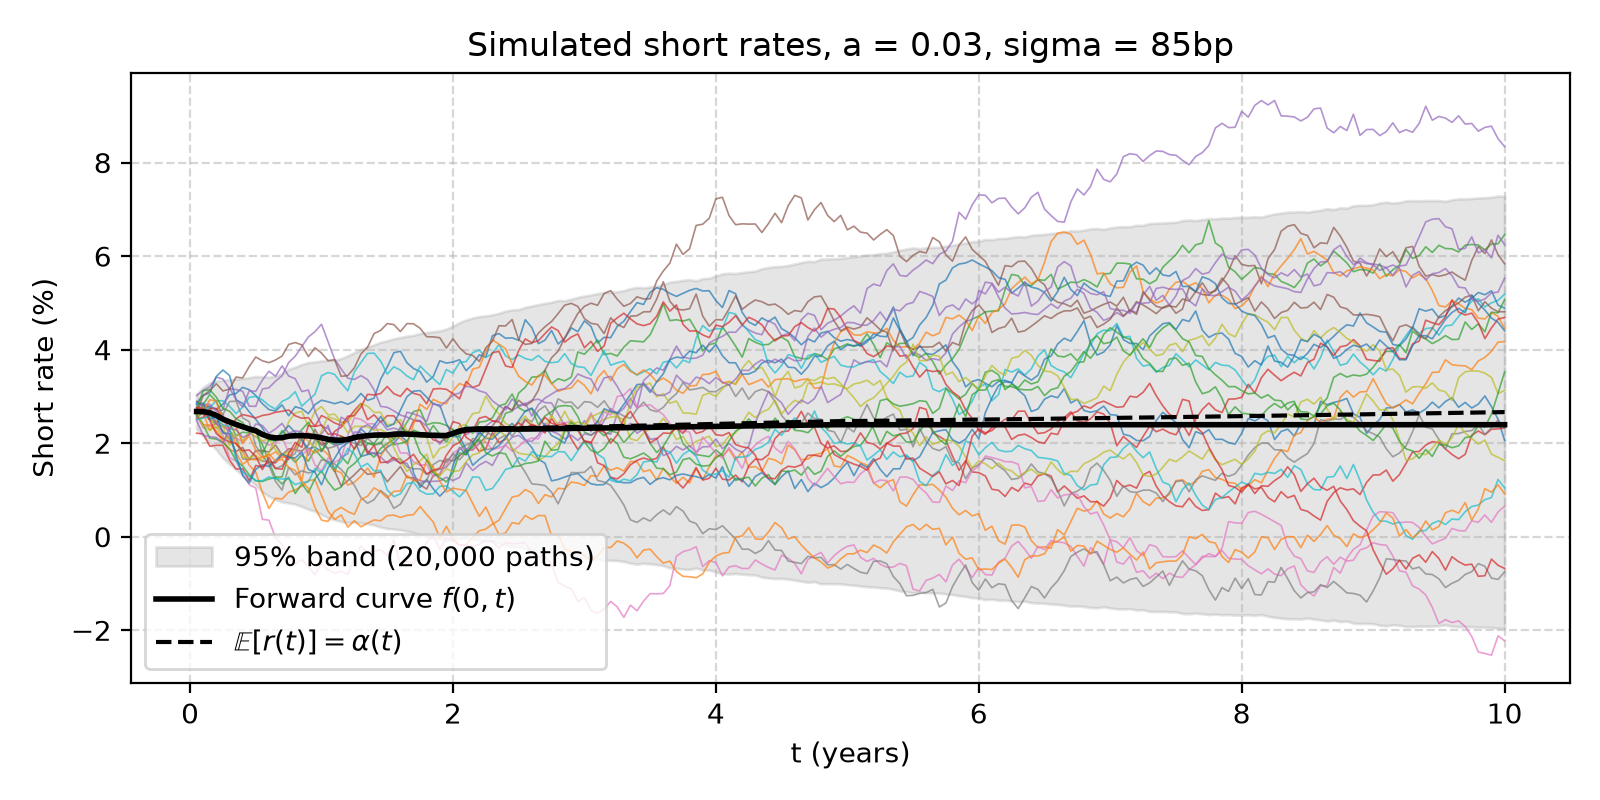
\includegraphics[width=0.85\textwidth]{short_rate_paths.png}
    \caption{Simulated short rates $r(t)=x(t)+\alpha(t)$ with $a=3\%$, $\sigma=85\bp$, initial forward curve and expected short rate.}
    \label{fig:paths}
\end{figure}

Figure~\ref{fig:alpha} shows $\alpha(t)$ and $\theta(t)$ for three mean reversions. The convexity term in $\alpha$ reaches $33\bp$ at 10 years for $a=1\%$ and $14\bp$ for $a=10\%$. The right panel illustrates Remark~\ref{rem:smooth}: even with the monotone convex interpolation, whose forward curve is continuous, $\theta$ oscillates between $-1.5\%$ and $+1.7\%$ per year over the first two years, because it inherits the slope of the forward curve between the short pillars. A scheme written in terms of $\theta$, such as a naive Euler discretization of~\eqref{eq:hw}, would be exposed to these oscillations; the shift decomposition is not.

\begin{figure}[htbp]
    \centering
    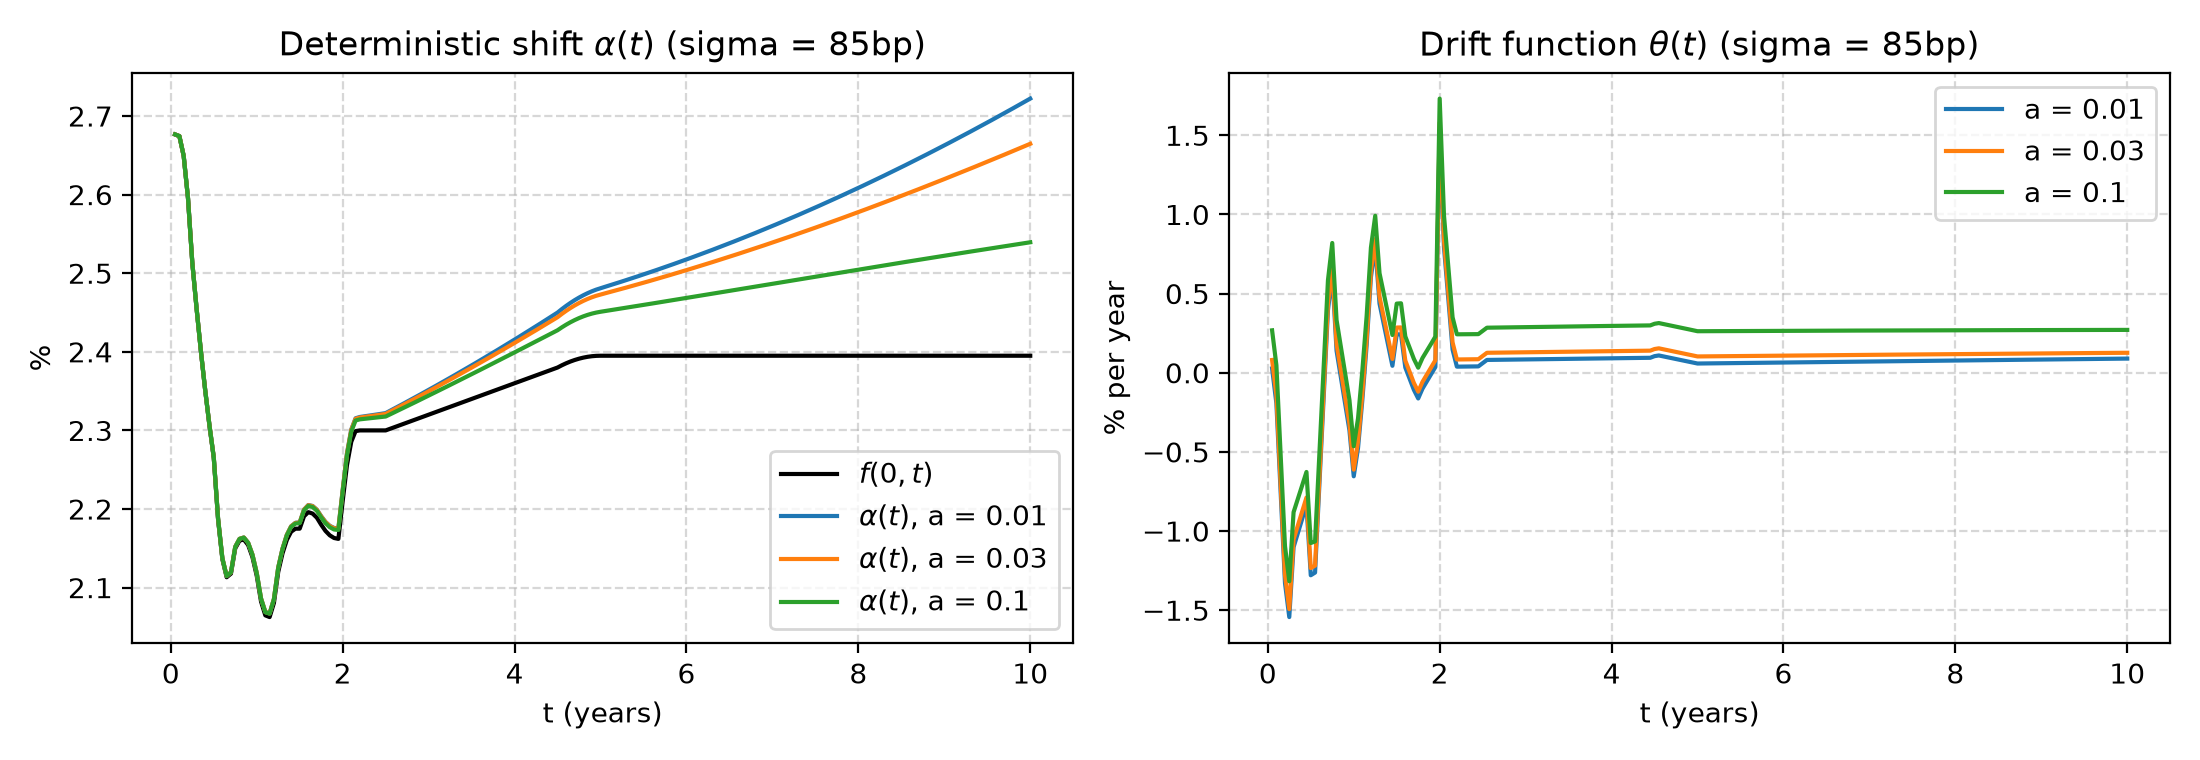
\includegraphics[width=\textwidth]{alpha_theta.png}
    \caption{Left: deterministic shift $\alpha(t)$ against the forward curve. Right: drift function $\theta(t)$.}
    \label{fig:alpha}
\end{figure}

\subsection{Volatility structure}
Figure~\ref{fig:caplets} shows the implied normal volatility of at-the-money 6M caplets as a function of the fixing date. As predicted by~\eqref{eq:caplet-vol}, $\sigma$ scales the whole curve, and $a$ controls its decay: almost flat for $a=0.1\%$, from $78\bp$ to $41\bp$ between 0.5 and 9.5 years for $a=20\%$. For $a=20\%$ and a fixing at 9.5 years, formula~\eqref{eq:caplet-vol} gives $85\times0.952\times0.507\approx41\bp$, in agreement with the exact price. No choice of constant parameters produces an increasing or humped term structure.

\begin{figure}[htbp]
    \centering
    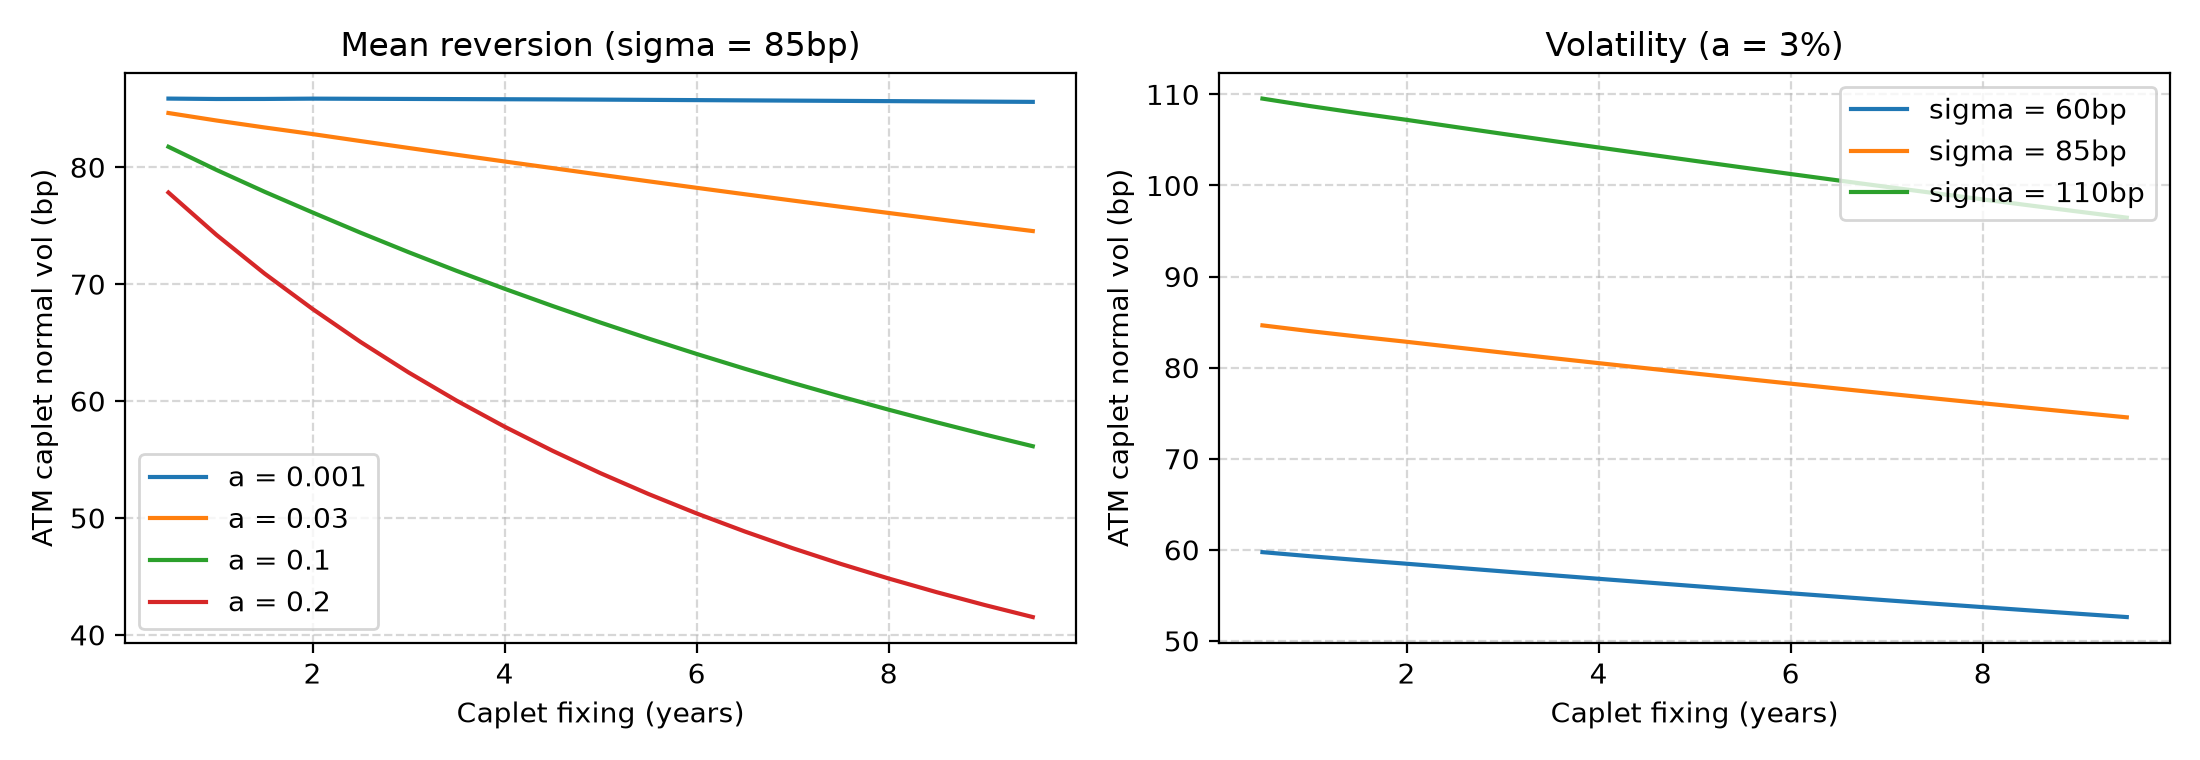
\includegraphics[width=\textwidth]{caplet_vols.png}
    \caption{Implied normal volatility of ATM 6M caplets. Left: effect of $a$; right: effect of $\sigma$.}
    \label{fig:caplets}
\end{figure}

Because all rates are driven by one factor, the 1-year and 10-year zero rates in 5 years are both affine in $x(5)$: their simulated correlation is exactly $1.000000$ for every $a$. Only their relative volatility depends on $a$: the ratio of their standard deviations is $1.005$, $1.140$ and $1.505$ for $a=0.1\%$, $3\%$ and $10\%$, i.e.\ $\frac{B(5,6)}{1}\big/\frac{B(5,15)}{10}$.

Figure~\ref{fig:smile} shows the implied normal volatility of a caplet fixing in 5 years across strikes from $-200$ to $+200\bp$ around the forward ($2.41\%$). It varies only between $79.0$ and $79.8\bp$: a Gaussian model produces an almost flat smile in normal volatility. Market smiles, which are skewed and convex, cannot be reproduced.

\begin{figure}[htbp]
    \centering
    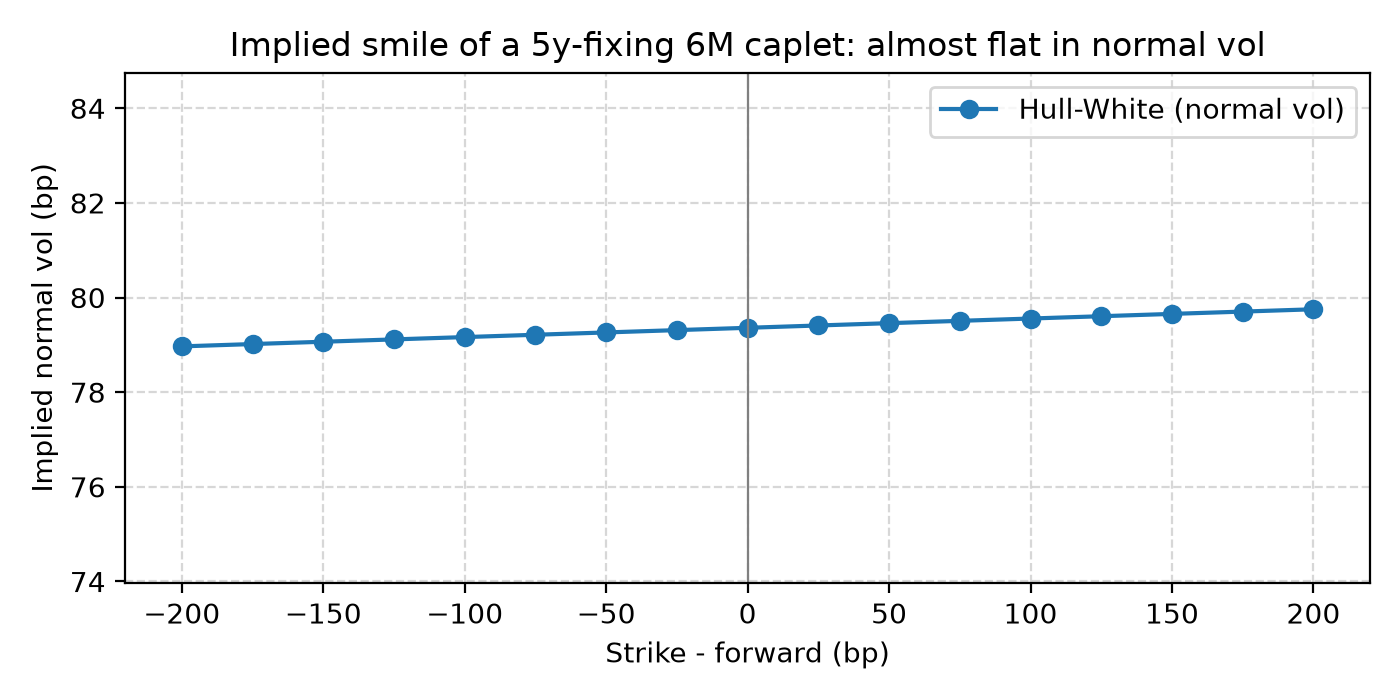
\includegraphics[width=0.7\textwidth]{smile.png}
    \caption{Hull--White implied normal volatility of a 6M caplet fixing in 5 years, as a function of the strike.}
    \label{fig:smile}
\end{figure}

\subsection{Calibration to a swaption grid}
We calibrate $(a,\sigma)$ to the 25 at-the-money European swaptions of the illustrative grid (expiries 0.5 to 5 years, tenors 1 to 10 years). The optimizer returns $a=0.23\%$ and $\sigma=77.2\bp$, with a root-mean-square error of $2.9\bp$ and a maximum error of $8.8\bp$ on the $0.5\text{y}\times1\text{y}$ swaption (Figure~\ref{fig:calibration}). The illustrative surface is humped in the expiry direction, rising from $70\bp$ at 6 months to $82\bp$ at 2--3 years, as is typical of EUR markets. With constant parameters the model can only produce volatilities that decrease with the expiry, so the optimizer pushes $a$ to almost zero and produces an almost flat surface around $78\bp$: it overprices short expiries and underprices the 2--3 year expiries, with a structured error pattern rather than noise.

\begin{figure}[htbp]
    \centering
    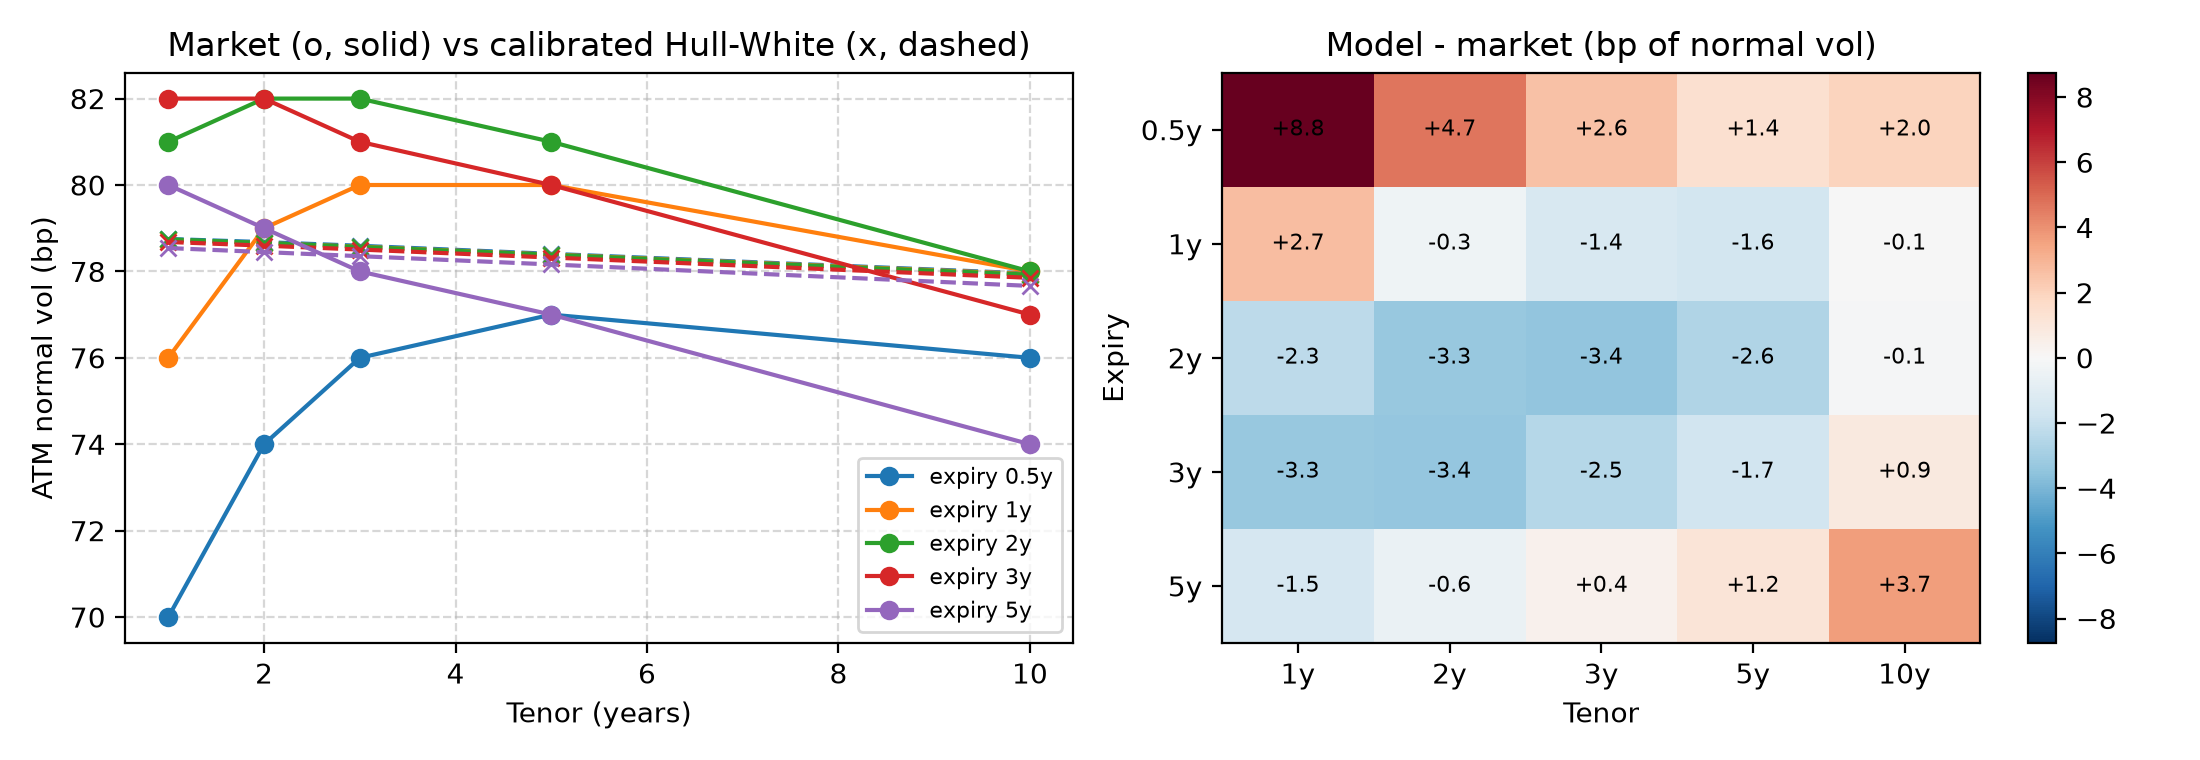
\includegraphics[width=\textwidth]{calibration.png}
    \caption{Global calibration to 25 ATM swaptions. Left: market and model normal volatilities; right: errors in bp.}
    \label{fig:calibration}
\end{figure}

A co-terminal calibration to the nine swaptions $T_k\times(10-T_k)$, $T_k=1,\dots,9$, is far better: $a=8.9\%$, $\sigma=115.3\bp$, RMSE $0.58\bp$ and maximum error $0.96\bp$. The model is good at fitting a one-dimensional slice of the surface, not the whole surface. Note that the two calibrations give very different parameters ($a$ from $0.2\%$ to $8.9\%$): the parameters of HW1F are not intrinsic quantities, they depend on the instruments chosen.

\subsection{Bermudan swaption and the role of mean reversion}
\label{sec:bermudan-num}
We price a $2\text{y}\times8\text{y}$ payer Bermudan swaption (notional 1 million euros, annual fixed leg, exercisable every year from 2 to 9 years into the remaining swap ending at 10 years), struck at the forward swap rate $K=2.4013\%$, with 200{,}000 Longstaff--Schwartz paths. With the co-terminal calibration above, its price is $46{,}441\pm58\,\eur$, against $32{,}417\,\eur$ for the most expensive co-terminal European swaption ($3\text{y}\times7\text{y}$). The option to choose the exercise date is worth about $14{,}000\,\eur$, or $43\%$ of the best European. The holder exercises at the first date on $20.9\%$ of the paths, and never on $27.4\%$. As a check, the Monte Carlo price of the $2\text{y}\times8\text{y}$ European swaption ($30{,}337\,\eur$) agrees with the closed form~\eqref{eq:jamshidian} ($30{,}409\,\eur$) within the statistical error.

Table~\ref{tab:bermudan} repeats the exercise with $a$ fixed at three levels and $\sigma$ calibrated to the same co-terminal swaptions. All three calibrations fit the European swaptions within $1\bp$, and the most expensive European barely moves ($32{,}355$ to $32{,}611\,\eur$). Yet the Bermudan price moves from $43{,}029$ to $46{,}841\,\eur$, i.e.\ by $9\%$, and the switch option by $39\%$.

\begin{table}[htbp]
\centering
\small
\begin{tabular}{@{}rrrrrr@{}}
\toprule
$a$ (fixed) & $\sigma$ (bp) & RMSE (bp) & Max European (\eur) & Bermudan (\eur) & Switch option (\eur) \\
\midrule
0.1\% & 77.0  & 0.88 & 32{,}611 & 43{,}029 & 10{,}418 \\
3\%   & 88.5  & 0.83 & 32{,}609 & 44{,}174 & 11{,}565 \\
10\%  & 120.7 & 0.61 & 32{,}355 & 46{,}841 & 14{,}486 \\
\bottomrule
\end{tabular}
\caption{$2\text{y}\times8\text{y}$ payer Bermudan swaption ATM, notional 1M\eur, with $a$ fixed and $\sigma$ calibrated to the co-terminal swaptions. Monte Carlo standard error about $60\,\eur$.}
\label{tab:bermudan}
\end{table}

The explanation is the intertemporal correlation of Section~\ref{sec:bonds}. The value of the right to wait depends on how much the forward swap rates seen at different exercise dates decorrelate: the more they decorrelate, the more information is gained by waiting. A higher $a$ lowers the correlation between $x(T_k)$ and $x(T_{k+1})$, and the higher $\sigma$ required to keep the European prices fixed increases the dispersion, so the Bermudan premium increases. European swaptions, each depending on the distribution of the state at a single date, cannot pin down this correlation. \emph{The mean reversion is the key unobservable parameter of Bermudan pricing}, and the price of a Bermudan in HW1F carries a model risk that must be managed explicitly (reserves, parameter stress tests, comparison with a two-factor model).

\clearpage
% ===============================================================
\section{Advantages of the Model}
\label{sec:advantages}
% ===============================================================

\paragraph{1. Exact fit to the initial curve.} By construction, $\theta$ (or $\alpha$) absorbs the whole curve, for any $(a,\sigma)$. Swaps, FRAs and bonds are priced at market, and options are priced consistently with their underlying forwards. This is the fundamental improvement over Vasicek and CIR.

\paragraph{2. Analytical tractability.} Zero-coupon bonds (Theorem~\ref{thm:bond}), bond options (Proposition~\ref{prop:zbo}), caps and floors~\eqref{eq:caplet} and European swaptions (Proposition~\ref{prop:jamshidian}) all have closed forms. Futures convexity adjustments, CMS-type approximations and many other quantities are also explicit. Calibration loops run in milliseconds.

\paragraph{3. Markovian in one dimension.} The whole curve at any date is a function of one Gaussian variable. Trees, one-dimensional PDEs and regression-based Monte Carlo are fast and accurate, which makes the model the natural choice for Bermudan swaptions, callable bonds, callable range accruals and other early-exercise products.

\paragraph{4. Exact and cheap simulation.} The joint law of $(x,\int x)$ is known (Section~\ref{sec:pricing}), so paths can be simulated without discretization bias and only at the dates of interest. Combined with the affine bond formula, this provides the full curve on every path at negligible cost, which is why HW1F is the default rate model in XVA, PFE and economic scenario generators.

\paragraph{5. Parsimony and interpretability.} Two parameters with a clear meaning: $\sigma$ is a level of normal volatility, $a$ the decay of volatility along the curve and the speed of decorrelation in time. Sensitivities are easy to interpret, and the model is easy to explain to traders, risk managers and validators.

\paragraph{6. Negative rates and normal volatilities.} The Gaussian distribution, long seen as a defect, became an asset when EUR, CHF and JPY rates turned negative in the 2010s. Lognormal models (Black--Karasinski, Black's formula) broke down, while HW1F needed no modification. It is consistent with the Bachelier (normal volatility) quotation that is now standard in rate option markets.

\paragraph{7. A building block.} Its simplicity makes HW1F the rate component of choice in hybrid models (Hull--White rates with Heston or local volatility equity, two Hull--White models with a correlated FX process), in which correlations between factors can be handled analytically.

\clearpage
% ===============================================================
\section{Drawbacks and Limitations}
\label{sec:drawbacks}
% ===============================================================

\paragraph{1. A single factor: perfectly correlated rates.} All rates are driven by one Brownian motion, so the instantaneous correlation between any two rates is one. The curve can only move by the deformation $T\mapsto B(t,T)$ scaled by a random number: no independent slope or curvature moves. A principal component analysis of historical curve moves (see the yield curve paper of this portfolio) attributes about $80\%$ of the variance to the level factor and the rest to slope and curvature, which HW1F ignores. Products that depend on the decorrelation between rates, such as CMS spread options, curve steepeners or spread range accruals, are \emph{mispriced by construction}: in HW1F a spread option between the 10-year and 2-year rates has essentially the volatility of a single rate multiplied by a deterministic factor.

\paragraph{2. Rigid volatility term structure.} With constant parameters, caplet and swaption volatilities decrease with expiry (equations~\eqref{eq:caplet-vol} and~\eqref{eq:swaption-vol}). Market surfaces are typically humped. Section~\ref{sec:numerics} shows the consequence: a structured RMSE of $2.9\bp$ on a modest illustrative grid, and a maximum error of $8.8\bp$. Two parameters cannot describe a two-dimensional surface.

\paragraph{3. No smile.} The model is Gaussian, so implied normal volatilities are almost flat in strike (Figure~\ref{fig:smile}). Market smiles are skewed and convex, and the skew moves with the level of rates. Out-of-the-money options, and products whose value depends on the smile (callable range accruals, digital caps, CMS products whose replication involves all strikes), are mispriced. In practice, desks calibrate HW1F to the swaptions struck at the relevant strike of each trade, which gives a different model for every product.

\paragraph{4. Negative rates without bound.} The other side of the Gaussian distribution: rates can become arbitrarily negative, with $12.8\%$ of short rates below zero at 10 years in our example. In a high-rate environment, or for products sensitive to the left tail (floors, zero-rate floors on deposits, inflation-linked floors), this probability may be unrealistic. The model is also unsuitable for markets where rates must stay positive by construction.

\paragraph{5. Unstable and non-intrinsic parameters.} The calibrated $a$ depends heavily on the instruments: $0.2\%$ on the global grid and $8.9\%$ on the 10-year co-terminals in our example. It is often poorly identified, with flat objective functions, and jumps from day to day, which produces noisy hedge ratios and P\&L. The time-dependent drift $\theta$ also means that the model is re-fitted every day to a new curve: the dynamics implied today are not consistent with the dynamics implied tomorrow.

\paragraph{6. Mean-reversion model risk for multi-exercise products.} As shown in Table~\ref{tab:bermudan}, the Bermudan premium depends on $a$, which European options barely constrain. The model gives one number for the intertemporal correlation, determined indirectly by the shape of the volatility surface, not by market information on that correlation.

\paragraph{7. Sensitivity to the curve construction.} Through $\theta$, the model depends on the derivative of the forward curve (Remark~\ref{rem:smooth}). A poor interpolation produces a jagged drift, unrealistic short-rate dynamics and noisy sensitivities. The shift formulation reduces the problem but does not remove the dependence on the instantaneous forward curve.

\paragraph{8. Single-curve setting.} The basic model describes one curve used both for discounting and for projection. Since 2008 the market uses several curves (OIS for discounting, EURIBOR 3M, 6M for projection, and today €STR and SOFR term rates). Extending HW1F requires deterministic or stochastic basis spreads between the curves.

\paragraph{9. Unrealistic historical dynamics.} Calibrated under $\Q$ to option prices, the model says little about the real-world distribution of rates. Historical rates show volatility clustering, regime changes and a level-dependent volatility, none of which is captured. The model is a pricing tool, not a forecasting tool.

\clearpage
% ===============================================================
\section{Extensions}
\label{sec:extensions}
% ===============================================================

Each drawback of Section~\ref{sec:drawbacks} has a standard remedy, at the cost of some of the advantages of Section~\ref{sec:advantages}.

\paragraph{Time-dependent parameters.} With $\sigma(t)$ (and possibly $a(t)$) piecewise constant, the model keeps all its closed forms, with integrals replacing the exponentials. A piecewise constant $\sigma(t)$ can be bootstrapped to fit a strip of co-terminal swaptions exactly, one expiry after another, which is the market standard for Bermudans, and can reproduce a humped volatility term structure. The price is a less stationary volatility structure, since the future volatility surface implied by the model differs from today's.

\paragraph{The linear Gaussian model (LGM).} Hagan's LGM~\cite{hagan} is a reparametrization of HW1F with a time-dependent volatility, written in terms of a numéraire that makes the state variable a martingale. It is equivalent to Hull--White but numerically more robust, and is widely used in production systems.

\paragraph{Two factors: G2++.} The G2++ model~\cite{brigomercurio} writes $r(t)=x(t)+y(t)+\varphi(t)$ with two correlated Ornstein--Uhlenbeck processes. It is still Gaussian and affine, keeps the exact fit to the curve and closed forms for bonds, caps and (semi-analytically) swaptions, and introduces an imperfect correlation between rates and a humped volatility structure. It is equivalent to the two-factor Hull--White model and is the natural upgrade for spread products and for checking Bermudan model risk.

\paragraph{Smile: quasi-Gaussian and stochastic volatility.} The Cheyette (quasi-Gaussian) models~\cite{cheyette, andersenpiterbarg} replace $\sigma$ by a local volatility $\sigma(t,x)$, typically affine in the rate (a displaced diffusion), and possibly add a stochastic variance. They keep a low-dimensional Markov state and can fit the smile of the relevant swaptions, at the cost of losing exact closed forms for swaptions.

\paragraph{Positive rates: Black--Karasinski and CIR++.} Modelling $\ln r$ as a Hull--White process (Black--Karasinski~\cite{bk}) gives positive, lognormal rates, but no closed form for bonds, and a fit to the curve by numerical shifting. The CIR++ model of Brigo and Mercurio adds a deterministic shift to a CIR process. These models were abandoned for EUR and CHF during the negative rate period, but remain relevant for credit intensities.

\paragraph{Market models.} The LIBOR Market Model and its SABR variants model the observable forward rates directly, with rich correlation and smile structures. They are the reference for exotic products with strong dependence on the correlation or on the smile, but are high-dimensional and require Monte Carlo methods for early exercise.

\clearpage
% ===============================================================
\section{Conclusion}
\label{sec:conclusion}
% ===============================================================

The one-factor Hull--White model achieves a remarkable compromise. Starting from the Vasicek dynamics, the single time-dependent drift $\theta(t)$ makes the model consistent with today's yield curve, while preserving a Gaussian affine structure in one state variable. As a result, zero-coupon bonds, bond options, caps, floors and European swaptions have closed forms, the curve can be simulated exactly at any date, and early-exercise products can be priced with fast one-dimensional methods. The two parameters have a transparent meaning: $\sigma$ sets the level of normal volatility and $a$ its decay along the curve and its decorrelation over time.

The same simplicity is the source of its limitations. One factor means perfectly correlated rates; two constant parameters mean a monotone volatility term structure and an imperfect fit of the swaption surface; Gaussian rates mean no smile and unbounded negative rates. The numerical experiments of this paper make these points concrete: a co-terminal calibration fits within $1\bp$ but a global one leaves structured errors of up to $9\bp$; implied smiles are flat; and for a Bermudan swaption, equally good calibrations to European prices give prices $9\%$ apart, because the mean reversion that drives the switch option is not observed in European prices.

HW1F should therefore be seen as the right model for the right products: vanilla-like and callable products whose value depends mainly on the level of rates and on the volatility of one slice of the surface, risk simulations where speed matters more than smile accuracy, and as a benchmark and a building block. For products that depend on the decorrelation of rates or on the smile, it must be replaced or complemented by G2++, quasi-Gaussian or market models, and its key unobservable parameter, the mean reversion, must always be treated as a source of model risk.

\clearpage
\appendix
% ===============================================================
\section{Proofs}
\label{app:proofs}
% ===============================================================

\subsection{Distribution of the integrated short rate}
By Proposition~\ref{prop:shift}, $\int_t^Tr(u)\,\dd u=\int_t^Tx(u)\,\dd u+\int_t^T\alpha(u)\,\dd u$. Integrating~\eqref{eq:solution} for $x$ (with $\theta=0$) and exchanging the integrals,
\begin{equation}
    \int_t^Tx(u)\,\dd u=B(t,T)\,x(t)+\sigma\int_t^TB(u,T)\,\dd W(u).
\end{equation}
Conditionally on $\F_t$, it is Gaussian with mean $B(t,T)x(t)$ and variance
\begin{equation}
    \mathcal{V}(t,T)=\sigma^2\int_t^TB(u,T)^2\,\dd u=\frac{\sigma^2}{a^2}\Bigl(T-t-2\frac{1-e^{-a(T-t)}}{a}+\frac{1-e^{-2a(T-t)}}{2a}\Bigr).
    \label{eq:calV}
\end{equation}

\subsection{Proof of Theorem~\ref{thm:bond}}
Since $\E[e^{-Y}]=e^{-\E Y+\frac12\Var Y}$ for a Gaussian $Y$,
\begin{equation}
    P(t,T)=\exp\Bigl(-\int_t^T\alpha(u)\,\dd u-B(t,T)x(t)+\tfrac12\mathcal{V}(t,T)\Bigr).
    \label{eq:bond-raw}
\end{equation}
At $t=0$, $x(0)=0$, and exact fit requires $\exp(-\int_0^T\alpha+\frac12\mathcal{V}(0,T))=P(0,T)$ for all $T$, i.e.\ $\int_0^T\alpha=-\ln P(0,T)+\frac12\mathcal{V}(0,T)$. Differentiating in $T$ gives $\alpha(T)=f(0,T)+\frac12\partial_T\mathcal{V}(0,T)=f(0,T)+\frac{\sigma^2}{2}\cdot2\int_0^TB(u,T)e^{-a(T-u)}\,\dd u=f(0,T)+\frac{\sigma^2}{2a^2}(1-e^{-aT})^2$, which is~\eqref{eq:alpha}; Proposition~\ref{prop:shift} then gives~\eqref{eq:theta}, proving Proposition~\ref{prop:theta} (the converse follows since $\alpha$ is uniquely determined). Substituting $\int_t^T\alpha=\int_0^T\alpha-\int_0^t\alpha$ into~\eqref{eq:bond-raw},
\begin{equation}
    P(t,T)=\frac{P(0,T)}{P(0,t)}\exp\Bigl(-B(t,T)x(t)-\tfrac12\bigl[\mathcal{V}(0,T)-\mathcal{V}(0,t)-\mathcal{V}(t,T)\bigr]\Bigr),
\end{equation}
and a direct computation shows that $\frac12[\mathcal{V}(0,T)-\mathcal{V}(0,t)-\mathcal{V}(t,T)]$ equals $V(t,T)$ in~\eqref{eq:V}. Finally, replacing $x(t)=r(t)-\alpha(t)$ gives~\eqref{eq:A}, since $B(t,T)\frac{\sigma^2}{2a^2}(1-e^{-at})^2$ cancels between $B\alpha(t)$ and $V(t,T)$.

\clearpage
% ===============================================================
\section{Implementation}
\label{app:code}
% ===============================================================

The model is implemented in the class \texttt{HullWhite} of \texttt{Fixed\_Income\_Models/hull\_white\_1F.py}. The bond formula~\eqref{eq:bond}--\eqref{eq:V} and the bond option~\eqref{eq:zbc}:
\begin{lstlisting}[style=pystyle]
def bond_price(self, t, T, x):
    """ P(t,T) given the state x(t) (vectorised in T and x). """
    a, s = self.a, self.sigma
    B = self.B(t, T)
    convexity = B * s**2 / (2 * a**2) * (1 - np.exp(-a * t))**2 + s**2 / (4 * a) * (1 - np.exp(-2 * a * t)) * B**2
    return self.curve.discount(T) / self.curve.discount(t) * np.exp(-B * x - convexity)

def bond_option(self, T, S, X, is_call=True):
    P_T, P_S = self.curve.discount(T), self.curve.discount(S)
    sigma_p = self.sigma * np.sqrt((1 - np.exp(-2 * self.a * T)) / (2 * self.a)) * self.B(T, S)
    h = np.log(P_S / (P_T * X)) / sigma_p + sigma_p / 2
    if is_call:
        return P_S * norm.cdf(h) - X * P_T * norm.cdf(h - sigma_p)
    return X * P_T * norm.cdf(-h + sigma_p) - P_S * norm.cdf(-h)
\end{lstlisting}

Jamshidian's decomposition~\eqref{eq:jamshidian}:
\begin{lstlisting}[style=pystyle]
def european_swaption_value(self, swaption):
    T0 = swaption.expiry
    times, coupons = self._swaption_cashflows(swaption, T0)
    bond = lambda x: float(np.sum(coupons * self.bond_price(T0, times, x))) - 1.0
    x_star = brentq(bond, -2.0, 2.0, xtol=1e-14)
    strikes = self.bond_price(T0, times, x_star)
    options = self.bond_option(T0, times, strikes, is_call=not swaption.payer)
    return float(swaption.notional * np.sum(coupons * options))
\end{lstlisting}

The exact simulation step~\eqref{eq:exact} of $(x,\int x)$:
\begin{lstlisting}[style=pystyle]
e1, e2 = np.exp(-a * h), np.exp(-2 * a * h)
v11 = s**2 * (1 - e2) / (2 * a)
v22 = s**2 / a**2 * (h - 2 * (1 - e1) / a + (1 - e2) / (2 * a))
v12 = s**2 / (2 * a**2) * (1 - e1)**2
L = np.linalg.cholesky(np.array([[v11, v12], [v12, v22]]) + 1e-18 * np.eye(2))
eps = L @ Z
integral = integral + x * (1 - e1) / a + eps[1]
x = x * e1 + eps[0]
\end{lstlisting}

The calibration minimizes~\eqref{eq:calib} with \texttt{scipy.optimize.least\_squares}, and \texttt{bermudan\_swaption} implements the Longstaff--Schwartz algorithm on the exact simulation, with the exercise value of the remaining swap computed in closed form from $x(T_k)$.

\clearpage
% ===============================================================
\section{Notation}
\label{app:notation}
% ===============================================================

\begin{table}[htbp]
\centering
\small
\begin{tabular}{@{}ll@{}}
\toprule
Symbol & Meaning \\
\midrule
$r(t)$ & Instantaneous short rate \\
$\beta(t),\ D(t,T)$ & Bank account and stochastic discount factor \\
$P(t,T)$ & Price at $t$ of a zero-coupon bond maturing at $T$ \\
$f(t,T),\ F(t;T_1,T_2)$ & Instantaneous and simply compounded forward rates \\
$\Q,\ \Q^T$ & Risk-neutral and $T$-forward measures \\
$a,\ \sigma$ & Mean reversion speed and normal volatility of the short rate \\
$\theta(t)$ & Time-dependent drift fitted to the curve \\
$x(t),\ \alpha(t)$ & Centred Ornstein--Uhlenbeck factor and deterministic shift, $r=x+\alpha$ \\
$B(t,T)$ & $(1-e^{-a(T-t)})/a$ \\
$V(t,T),\ \mathcal{V}(t,T)$ & Convexity term of the bond formula, variance of $\int_t^Tx$ \\
$\sigma_P$ & Log-volatility of the bond $P(T,S)$ at the option expiry $T$ \\
$\mathrm{ZBC},\ \mathrm{ZBP}$ & Zero-coupon bond call and put \\
$A(t),\ S(t)$ & Annuity and forward swap rate \\
$c_i,\ x^*,\ X_i$ & Coupons, critical state and strikes of Jamshidian's decomposition \\
$\sigma_N$ & Implied normal (Bachelier) volatility \\
\bottomrule
\end{tabular}
\caption{Main notation.}
\label{tab:notation}
\end{table}

\clearpage

% ===============================================================
\begin{thebibliography}{99}
% ===============================================================

\bibitem{hullwhite}
J. Hull and A. White,
\textit{Pricing interest-rate-derivative securities},
Review of Financial Studies, 3(4):573--592, 1990.

\bibitem{hullwhite94}
J. Hull and A. White,
\textit{Numerical procedures for implementing term structure models I: single-factor models},
Journal of Derivatives, 2(1):7--16, 1994.

\bibitem{vasicek}
O. Vasicek,
\textit{An equilibrium characterization of the term structure},
Journal of Financial Economics, 5(2):177--188, 1977.

\bibitem{cir}
J. C. Cox, J. E. Ingersoll and S. A. Ross,
\textit{A theory of the term structure of interest rates},
Econometrica, 53(2):385--407, 1985.

\bibitem{holee}
T. S. Y. Ho and S.-B. Lee,
\textit{Term structure movements and pricing interest rate contingent claims},
Journal of Finance, 41(5):1011--1029, 1986.

\bibitem{hjm}
D. Heath, R. Jarrow and A. Morton,
\textit{Bond pricing and the term structure of interest rates: a new methodology for contingent claims valuation},
Econometrica, 60(1):77--105, 1992.

\bibitem{jamshidian}
F. Jamshidian,
\textit{An exact bond option formula},
Journal of Finance, 44(1):205--209, 1989.

\bibitem{geman}
H. Geman, N. El Karoui and J.-C. Rochet,
\textit{Changes of numéraire, changes of probability measure and option pricing},
Journal of Applied Probability, 32(2):443--458, 1995.

\bibitem{longstaff}
F. A. Longstaff and E. S. Schwartz,
\textit{Valuing American options by simulation: a simple least-squares approach},
Review of Financial Studies, 14(1):113--147, 2001.

\bibitem{bk}
F. Black and P. Karasinski,
\textit{Bond and option pricing when short rates are lognormal},
Financial Analysts Journal, 47(4):52--59, 1991.

\bibitem{cheyette}
O. Cheyette,
\textit{Markov representation of the Heath--Jarrow--Morton model},
SSRN Working Paper 6073, 1992.

\bibitem{hagan}
P. S. Hagan,
\textit{Evaluating and hedging exotic swap instruments via LGM},
Bloomberg Technical Report, 2002.

\bibitem{haganwest2006}
P. S. Hagan and G. West,
\textit{Interpolation methods for curve construction},
Applied Mathematical Finance, 13(2):89--129, 2006.

\bibitem{brigomercurio}
D. Brigo and F. Mercurio,
\textit{Interest Rate Models -- Theory and Practice},
2nd edition, Springer Finance, 2006.

\bibitem{andersenpiterbarg}
L. B. G. Andersen and V. V. Piterbarg,
\textit{Interest Rate Modeling, Volumes I--III},
Atlantic Financial Press, 2010.

\end{thebibliography}

\end{document}
